\textbf{Pour cette première partie, aucune justification n'est demandée et une seule réponse est possible par question. Pour chaque question, reporter son numéro sur la copie et indiquer la réponse.}

Une réponse fausse ou l'absence de réponse n'enlève aucun point.

\subsection*{Question 1}

Le nombre $3^4 \times 3^2$ est égal à :

\medskip
\begin{tblr}{colspec = {@{}*{4}{X}}}
	\textbf{A.}\quad $3^8$ &
	\textbf{B.}\quad $3^6$ &
	\textbf{C.}\quad $9^6$ &
	\textbf{D.}\quad $27^5$ \\
\end{tblr}

\subsection*{Question 2}

On considère la droite passant par les points $A(1 ; 2)$ et $B(3 ; 6)$.

Son coefficient directeur est égal à :

\medskip
\begin{tblr}{colspec = {@{}*{4}{X}}}
	\textbf{A.}\quad 1 &
	\textbf{B.}\quad 2 &
	\textbf{C.}\quad 3 &
	\textbf{D.}\quad 4 \\
\end{tblr}

\subsection*{Question 3}

\begin{minipage}[t]{0.34\linewidth}
	On considère le graphique ci-contre qui donne le taux de pauvreté en pourcentage en France en fonction des années.

	\medskip

	Déterminer les années pour lesquelles le taux de pauvreté était de 14,5\,\%.

	\medskip
	\begin{tblr}{colspec = {@{}X}}
		\textbf{A.}\quad 2012 et 2015 \\
		\textbf{B.}\quad 2013 et 2020 \\
		\textbf{C.}\quad 2018 et 2021 \\
		\textbf{D.}\quad 2018, 2021 et 2023 \\
	\end{tblr}
\end{minipage}
\hfill
\begin{minipage}[t]{0.63\linewidth}
	\centering
	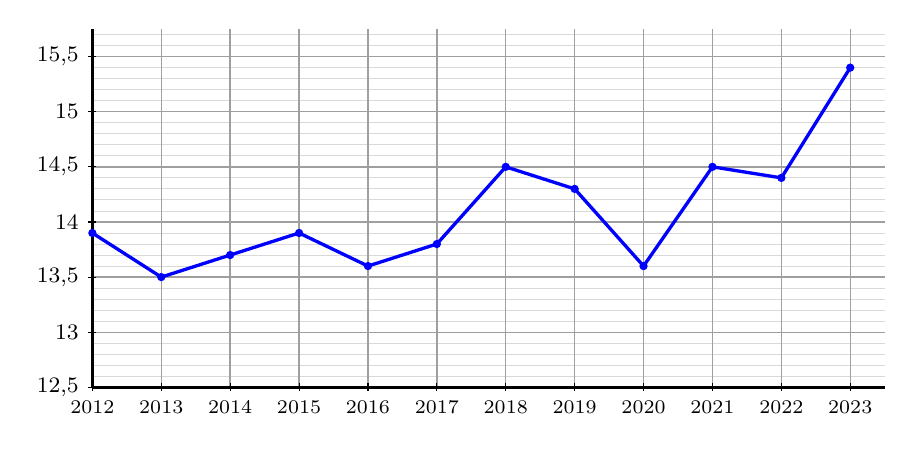
\begin{tikzpicture}[scale=0.7,x=1.25cm,y=2cm,>=stealth,baseline={(current bounding box.north)}]
		\draw[xstep=1,ystep=0.1,gray!30,line width=0.3pt] (0,0) grid (11.5,3.25);
		\draw[xstep=1,ystep=0.5,gray!75,line width=0.5pt] (0,0) grid (11.5,3.25);
		\draw[line width=1pt] (0,0) -- (11.5,0);
		\draw[line width=1pt] (0,0) -- (0,3.25);
		\foreach \x [count=\i from 0] in {2012,2013,...,2023} \draw (\i,2pt) -- (\i,-2pt) node[below] {\scriptsize \x};
		\foreach \y/\t in {0/{12,5},0.5/13,1/{13,5},1.5/14,2/{14,5},2.5/15,3/{15,5}} \draw (2pt,\y) -- (-2pt,\y) node[left] {\footnotesize \t};
		\draw[line width=1.2pt,blue] (0,1.4) -- (1,1.0) -- (2,1.2) -- (3,1.4) -- (4,1.1) -- (5,1.3) -- (6,2.0) -- (7,1.8) -- (8,1.1) -- (9,2.0) -- (10,1.9) -- (11,2.9);
		\foreach \x/\y in {0/1.4,1/1.0,2/1.2,3/1.4,4/1.1,5/1.3,6/2.0,7/1.8,8/1.1,9/2.0,10/1.9,11/2.9} \fill[blue] (\x,\y) circle (2.15pt);
	\end{tikzpicture}

	\emph{Source : Insee}
\end{minipage}

\subsection*{Question 4}

La forme développée et réduite de $(x-5)^2$ est :

\medskip
\begin{tblr}{colspec = {@{}*{4}{X}}}
	\textbf{A.}\quad $x^2 - 25$ &
	\textbf{B.}\quad $x^2 + 25$ &
	\textbf{C.}\quad $x^2 - 10x + 25$ &
	\textbf{D.}\quad $x^2 + 10x + 25$ \\
\end{tblr}

\subsection*{Question 5}

On considère la série de notes suivante : 14 ; 11 ; 11 ; 4 ; 10.

La moyenne est :

\medskip
\begin{tblr}{colspec = {@{}*{4}{X}}}
	\textbf{A.}\quad 11 &
	\textbf{B.}\quad 10,5 &
	\textbf{C.}\quad 10 &
	\textbf{D.}\quad 8 \\
\end{tblr}

\subsection*{Question 6}

\begin{minipage}[t]{0.6\linewidth}
	La fonction affine représentée dans le repère ci-contre est :

	\medskip
	\begin{tblr}{colspec = {@{}X}, rowsep=3pt}
		\textbf{A.}\quad $f(x) = -2x+3$ \\
		\textbf{B.}\quad $f(x) = -\dfrac{2}{3}x+3$ \\
		\textbf{C.}\quad $f(x) = \dfrac{3}{2}x+3$ \\
		\textbf{D.}\quad $f(x) = \dfrac{2}{3}x+3$ \\
	\end{tblr}
\end{minipage}
\hfill
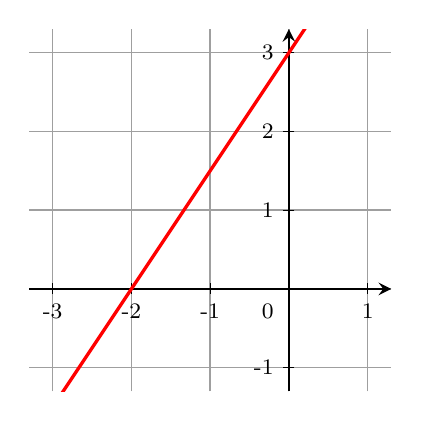
\begin{tikzpicture}[x=1cm,y=1cm,>=stealth,baseline={(current bounding box.north)}]
	\draw[step=1,gray!75,line width=0.5pt] (-3.3,-1.3) grid (1.3,3.3);
	\draw[->,line width=1pt] (-3.3,0) -- (1.3,0);
	\draw[->,line width=1pt] (0,-1.3) -- (0,3.3);
	\foreach \x in {-3,-2,-1,1} \draw (\x,2pt) -- (\x,-2pt) node[below] {\footnotesize \np{\x}};
	\foreach \y in {-1,1,2,3} \draw (2pt,\y) -- (-2pt,\y) node[left] {\footnotesize \np{\y}};
	\draw (-2pt,-2pt) node[below left] {\footnotesize 0};
	\clip (-3.3,-1.3) rectangle (1.3,3.3);
	\draw[line width=1.2pt,red] plot[domain=-3.3:1.3] (\x,{1.5*\x+3});
\end{tikzpicture}

\subsection*{Question 7}

Le tableau de signes de $f(x) = -10x+4$ est :

\medskip
\begin{tblr}{colspec = {@{}*{2}{X}}, rowsep=6pt}
	\textbf{A.}\quad
	\begin{tikzpicture}[baseline=(current bounding box.center)]
		\tkzTabInit[espcl=1.75]{$x$/0.8,$f(x)$/0.8}{$-\infty$,$-0{,}4$,$+\infty$}
		\tkzTabLine{,+,z,-,}
	\end{tikzpicture}
	&
	\textbf{B.}\quad
	\begin{tikzpicture}[baseline=(current bounding box.center)]
		\tkzTabInit[espcl=1.75]{$x$/0.8,$f(x)$/0.8}{$-\infty$,$-0{,}4$,$+\infty$}
		\tkzTabLine{,-,z,+,}
	\end{tikzpicture}
	\\
	\textbf{C.}\quad
	\begin{tikzpicture}[baseline=(current bounding box.center)]
		\tkzTabInit[espcl=1.75]{$x$/0.8,$f(x)$/0.8}{$-\infty$,$0{,}4$,$+\infty$}
		\tkzTabLine{,+,z,-,}
	\end{tikzpicture}
	&
	\textbf{D.}\quad
	\begin{tikzpicture}[baseline=(current bounding box.center)]
		\tkzTabInit[espcl=1.75]{$x$/0.8,$f(x)$/0.8}{$-\infty$,$0{,}4$,$+\infty$}
		\tkzTabLine{,-,z,+,}
	\end{tikzpicture}
	\\
\end{tblr}

\subsection*{Question 8}

Un prix est passé de 25~\euro{} à 20~\euro. Quel est le pourcentage de réduction ?

\medskip
\begin{tblr}{colspec = {@{}*{4}{X}}}
	\textbf{A.}\quad 20\,\% &
	\textbf{B.}\quad 25\,\% &
	\textbf{C.}\quad 5\,\% &
	\textbf{D.}\quad 10\,\% \\
\end{tblr}
